Nói sơ qua về hệ thống code thì ta sẽ giao tiếp trực tiếp trong cấu trúc của code chứ không nhập hàm số trong terminal vì dễ gây lỗi.

\subsection*{Khối đầu vào}
Ở đây code sẽ nhận vào các giá trị đầu vào là số biến của hệ, các hàm cần giải cho hệ, sai số dừng của hệ ở hình \ref{fig:sec4_1} 

\subsection*{Khối xử lý điều kiện đầu vào}
Lúc này ta sẽ cần phải tuyến tính hóa hệ phương trình bằng cách tính toán ma trận Jacobian của hệ phương trình bằng lệnh của MATLAB. Và ta gán biến symbolic vào hệ qua lệnh matlabFunction như ở hình \ref{fig:sec4_2}

\subsection*{Khối giải hệ tuyến tính}
Để phục vụ cho việc tính toán các dạng hệ phương trình tuyến tính khác nhau và để tối ưu thời gian, ở đây sẽ là nơi thiết lập các hàm như \textbf{lặp Jacobi, Gauss-Seidel, phương pháp phân rã LU} hình \ref{fig:sec4_3}

\subsection*{Khối lặp}
Từ giá trị $\mathbf{x^{(0)}}$ thì ta cần phải tính nghiệm $\Delta x_k$ lặp đi lặp lại qua công thức $J_k.\Delta x_k=-F(x_k)$ và dựa theo điều kiện dừng. Ở hình \ref{fig:sec4_4}

\begin{center}
\begin{figure}[H]\centering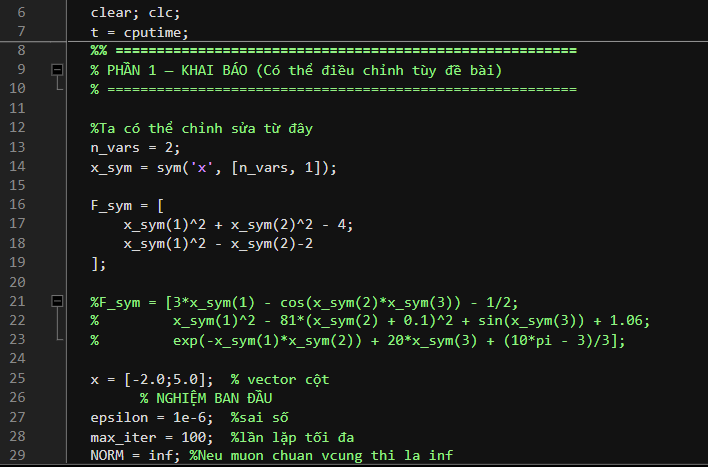
\includegraphics[width=0.6\linewidth]{pic/sec4_1.png}
\vspace{0.5cm}
\caption{Khối đầu vào}
\label{fig:sec4_1}
\end{figure}
\end{center}


\begin{center}\begin{figure}[H]\centering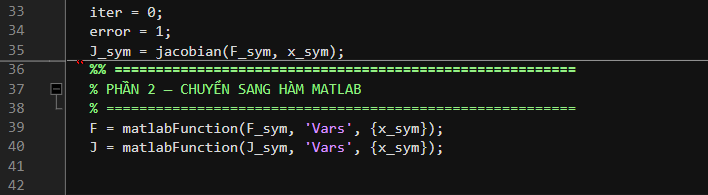
\includegraphics[width=0.7\linewidth]{pic/sec4_2.png}\vspace{0.5cm}\caption{Khối xử lý tín hiệu đầu vào}
\label{fig:sec4_2}\end{figure}\end{center}

\begin{center}\begin{figure}[H]\centering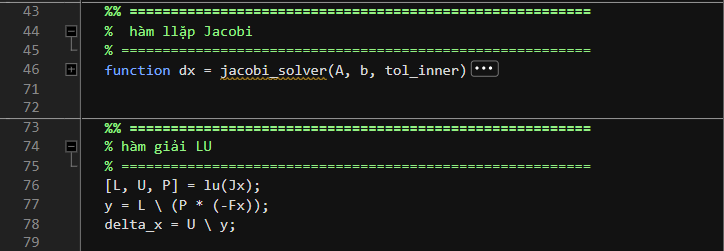
\includegraphics[width=0.7\linewidth]{pic/sec4_3.png}\vspace{0.5cm}\caption{Khối giải hệ tuyến tính}
\label{fig:sec4_3}\end{figure}\end{center}

\begin{center}\begin{figure}[H]\centering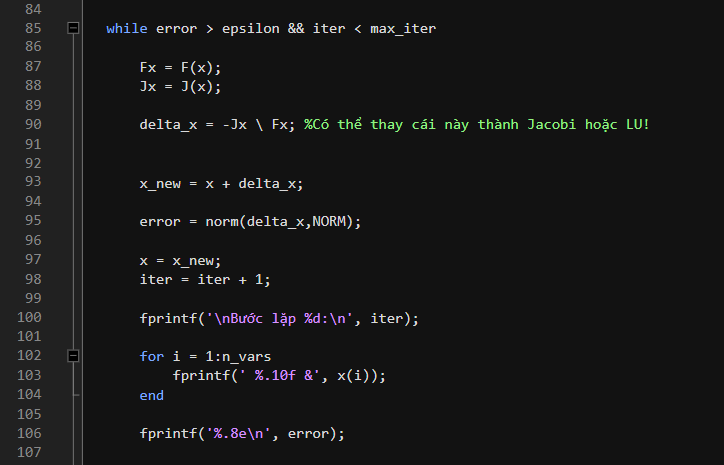
\includegraphics[width=0.7\linewidth]{pic/sec4_4.png}\vspace{0.5cm}\caption{Khối lặp}
\label{fig:sec4_4}\end{figure}\end{center}

\subsection*{ Khối xuất giá trị}

Khi này ta cần các giá trị xuất ra sẽ là ở hình \ref{fig:sec4_5}
\begin{itemize}
    \item Lần lặp $k$
    \item Nghiệm thứ nhất, thứ 2,.... đến nghiệm thứ $n$.
    \item Sai số nghiệm tại lần lặp đó $||\Delta x||$
\end{itemize} 
\begin{center}\begin{figure}[H]\centering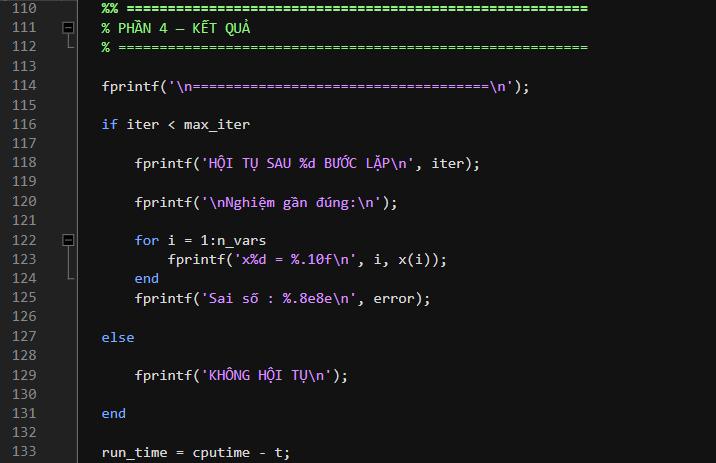
\includegraphics[width=0.7\linewidth]{pic/sec4_5.png}\vspace{0.5cm}\caption{Khối xuất giá trị}
\label{fig:sec4_5}\end{figure}\end{center}
